\documentclass[10pt,a4paper]{article}
\usepackage{times}
\usepackage{graphics}
\usepackage{graphicx}
\usepackage{natbib}
\usepackage{durhampaper}
\usepackage{subfigure}
\usepackage{todonotes}
% \usepackage{harvard}
% \usepackage[moderate]{savetrees}
\usepackage{url}

\title{Facial Liveness Testing: For The Web}
\author{} % leave; your name goes into \student{}
\student{Ryan Collins}
\supervisor{Prof A. Krokhin}
\degree{MEng Computer Science}

\date{\today}

\begin{document}

\maketitle

\begin{abstract}
% These instructions give you guidelines for preparing the final paper.  DO NOT change any settings, such as margins and font sizes.  Just use this as a template and modify the contents into your final paper.  Do not cite references in the abstract.

% The abstract must be a Structured Abstract with the headings {\bf Context/Background}, {\bf Aims}, {\bf Method}, {\bf Results}, and {\bf Conclusions}.  This section should not be longer than half of a page, and having no more than one or two sentences under each heading is advised.
\paragraph{Context}
    With password based authentication methods being subject to many attacks, facial recognition is an alternative, not relying on memory but instead
    on biometrics. However, with facial recognition comes face spoofing: methods to fool the algorithms into thinking one is someone different to who they are.
    In order for facial recognition to become more prevalent on the web, facial liveness is needed. With client side code comes the risk that the input could be tampered with,
    so server side services are ideal for security, and this leaves a few questions: what metrics are suitable for deploying in such a service, and how feasible is the construction of such a service?

\paragraph{Aims}
    % This might belong more in the method.
    \begin{itemize}
        \item Verify the results of the Image Quality Assessment test.
        \item Assess the outcome Convolutional Neural Networks on classifying real/spoofed images.
        \item Design and implement a new 3D based liveness test, aimed to prevent mask attacks.
        \item Determine the outcome of fusing the three above methods together, and how successful this is.
    \end{itemize}

\paragraph{Method}
   \begin{itemize}
        \item The image quality assessment test was implemented in Python to consider the image as a whole
        \item A CNN based 2D liveness test was implemented in Python to classify facial structure.
        \item A 3D based liveness test was proposed and investigated as to its usefulness.
   \end{itemize}
\paragraph{Results}
    \begin{itemize}
        \item Image Quality Assessment test performed well, being in the 90\% accuracy range over ReplayAttack test.
        \item CNN based 2D test performed adequately, yielding 76\% accuracy over the ReplayAttack test dataset.
        \item The VoxNet based 3D liveness test performed poorly, and had various performance issues that means it's not currently practical to deploy.
    \end{itemize}
\paragraph{Conclusions}
    Overall, both the Image Quality assessment and CNN based 2D test are ideal in a web-based liveness test as a service system. Image Quality based metric individually yields
    impressive results, but the CNN based metric would perform well when working together with other metrics. In addition, the speed at which queries can be answered shows 
    that these can reasonably be used in a web system without extensive delays in processing, or without requiring any additional hardware (aside from a camera).
\end{abstract}

\begin{keywords}
Facial liveness, convolutional neural networks, image quality metrics
\end{keywords}

\section{Introduction}
    % What is the project about?
    Currently, username and password authentication is commonplace throughout the web. However, username and password
    based authentication systems have a number of problems. Some common passwords can be broken using dictionary attacks,
    especially if they consist partially or entirely of a word in a standard dictionary. Furthermore, the process of shoulder surfing is possible (watching out
    for someone's password, and how they type it).

    % TODO this needs to be readjusted to make it sound more formal and clear.
   While there are different measures of detecting liveness, each method is specialised towards defending against a given attack. The aim of this project is to understand
   the existing liveness detection methods, which type of attack they aim to prevent, and how effective they are. Once this has been achieved, the aim shall be to bring
   each of these methods together, hopefully improving the effectiveness of such a system by encorporating multiple methods.

    % TODO might be worth explaining that we are focusing here on only images, rather than video. Explain why...

    In this context, we propose a novel new 3D-based liveness test, based on a two part approach: (i) VRN based 3D reconstruction (ii) VoxNet based 3D classification.
    We also confirm the success of the Image Quality Assessment method for Facial Liveness, and provide an improve
    % In this context, we propose 

\section{Related Work}
    % LIT REVIEW GOES HERE!
    As defined in \cite{FaceSpoofingAttacksStudy}, the types of face spoofing attacks can be described under three sections: Photo Attack, Video Attack and Mask Attack.

    \subsection{2D Spoofing Attacks}
        Photo and Video Attacks are both 2D spoofing attacks, which involve using a previously retrieved photo/video, and holding it in front of a camera. In the case of photo attacks,
        a single photo is used, where in video, some video would be played back on a screen. \cite{FaceSpoofingAttacksStudy}.

        With video-based facial recognition systems, motions of some form can be used to determine whether the person is real or spoofed, such as blinking, head movement and others.
        % TODO "As shown in ..., a blinking method using ... yields ... results
        % Head movement methods shown in .... yield ... by using ...
        % Face flashing methods, recently proposed in ..., yield impressive results, but require a screen and the results vary based on screen size.
        In the method defined in \cite{SFMClassifier}, structure from motion was used on the video to produce a 3D model of a user, with the depth channel being used to determine whether a person is real, or whether it's simply an image.
        They also extended this by fusing this method with audio verification. The fusion of multiple methods provides greater reliablity. However, while SFM works with video, it doesn't work with a single image,
        and it also doesn't work if a video with little motion is provided. This fusion was completed using a Bayesian Network 

        While motion based methods are video-only, quality based methods are useful for both videos and images (either by extracting key video frames or using all video frames and combining the results).
        %TODO explain old image quality methods, and their results and how they work. What's bad/what's good?

        While there are various quality metrics that have been used, combining a large number of them can yield some increased accuracy. By combining 25 different metrics,
        , yielding the resulting metric values into a large vector, and using that as input to a classifier (an LDA), this yields fairly high accuracy. \cite{ImageQualityAssessmentTest}.
        This is an example of combining many items to yield better results. While each metric on its own isn't that great, using them all together yields better results.
        
        Recently, deep learning based approaches have been applied to facial liveness (both video and image based).

        In particular, Convolutional Neural Networks are a key approach to this to learn features (e.g. texture based methods).
        Due to the existing datasets available, training CNNs has been difficult due to lack of data where overfitting has been common.
        The method proposed in \cite{Patel2016CrossDatabaseFA} uses CaffeNet, inputting both the full image along with the isolated face.
        The output yielded general texture differences, as well as specific facial texture differences. Another interesting idea proposed
        in this paper is the fusion of two algorithms together to produce an outcome, therefore reducing the false reject rate.
        %Cite above wiht http://vipl.ict.ac.cn/uploadfile/upload/2017020711382879.pdf
        
        \subsubsection{General 2D image classification models}
        Outside of the facial liveness field, image classification on the imagenet dataset has proven popular and yielded some fairly good
        results. 
        
        \paragraph{AlexNet} 
        One of the initial models was AlexNet, which has 5 convolutional layers (with some max pooling layers), and two globally connected layers.
        This model was used to classify 1.3 million high resolution images into 1000 classes. \cite{AlexNet} Overall deployability
        with Alexnet is fairly good due to a fairly low number of compute operations (meaning faster compute time). \cite{DeepNeuralNetworkDeployability} However, the accuracy of AlexNet isn't
        as good as newer methods (such as the ones shown below), which all perform better in terms of accuracy. 
        
        \paragraph{VGG16 Network}
        The VGG16 model improved AlexNet by replacing larger filters by more smaller filters one after another.
        However, VGG requires a high amount of computational power, something that's not easily deployable due to
        the large number of parameters (128 million), which requires a high amount of memory and compute power compared
        to other models. \cite{DeepNeuralNetworkDeployability}

        \paragraph{GoogLeNet Inception}
        GoogLeNet is an improved module that approximates a space Convolutional Network with a normal
        dense construction. One of the major features of GoogLeNet is the Inception module. The naive approach to this 
        is to take the input from the previous layer, calculate a 1x1, 3x3 and 5x5 convolution (all at the same time), along with
        a 3x3 max pooling before feeding this into an output, the output being the filter concatenation step.
        However, to reduce the diemsnionality, and therefore improve performance, a 1x1 convolution is applied before
        each 3x3 and 5x5 convolution, and after the max pooling output. These inception modules can be used and stacked
        to improve performance without a huge increase in computation. \cite{GoogLeNet} 
        This is shown in Figure \ref{InceptionArchitecture}.

        \begin{figure}
            \centering
            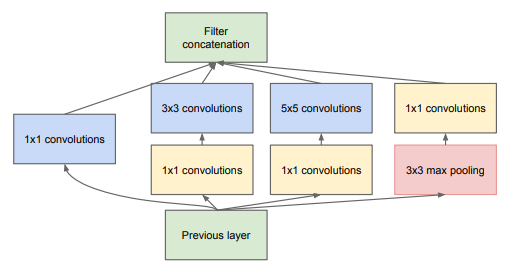
\includegraphics[width=0.7\linewidth]{InceptionModule.png}
            \caption{The Inception module with dimensionality reduction. Diagram taken from \cite{GoogLeNet}.}
            \label{InceptionArchitecture}
        \end{figure}

        Therefore, this model has improved computational performance over VGG, making it a more suitable model for the web compared to VGG. \cite{DeepNeuralNetworkDeployability}
        
        \paragraph{Residual Networks}
        Another key problem with deep convolutional networks on Image Classification is the vanishing gradient problem, where early layers have very small gradients during the training process and
        are therefore much more difficult to train. Residual Networks avoid this problem by allowing a direct path in links between the input and output of a building block. \todo{Explain Resnets better}.
        The overall outcome is far better accuracy than VGG and GoogLeNet while being more efficent than VGG in terms of computational power needed. \todo{Cite Residual Networks}
        While these aren't directly associated with facial liveness, the nature of image classification is fairly similar to facial liveness (since the image is simply a classifier with two outputs instead of 1000).
        
        In terms of Top-1\% accuracy (the accuracy with the top output in a multiclass problem) shown in Figure \ref{Top1AccuracyOverNetwork}, newer version of the Inception model perform the best,
        with ResNet based classifiers not too far behind. AlexNet performance was fairly poor. Now compare this with the operations (the required computational power for each model), which is shown in Figure \ref{Top1AccuracyOverOperations}.
        AlexNet and GoogLeNet require fairly few operations, in the $<10 GOps$ range. The same is true for smaller ResNet based models (e.g. ResNet 50 and 34).
        Meanwhile, VGG requires a fairly large amount of operations ($>30 GOps$), as do later versions of Inception.


        \begin{figure}
            \centering
            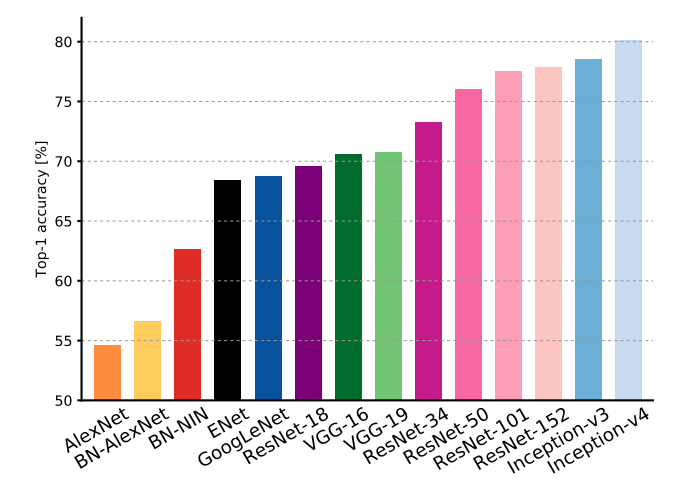
\includegraphics[width=.7\linewidth]{Top1AccuracyOverNetwork.png}
            \label{Top1AccuracyOverNetwork}
            \caption{Top 1 accuracy vs network. Chart and results from \cite{DeepNeuralNetworkDeployability}}
        \end{figure}

        \begin{figure}
            \centering
            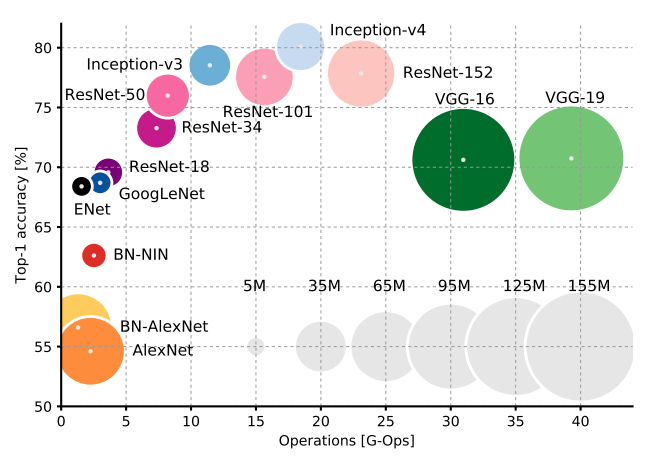
\includegraphics[width=.7\linewidth]{Top1AccuracyOverOperations.png}
            \label{Top1AccuracyOverOperations}
            \caption{Top 1 accuracy vs operations, where network size is proportional to parameters. Operations figures are for a single pass (e.g. predicting given a specific input). Chart and results from \cite{DeepNeuralNetworkDeployability}}
        \end{figure}

        \subsubsection{Datasets}
        %Datasets
        While models exist, in order to test these models data is needed. One of the most common and earliest dataset for facial liveness is the NUAA dataset,
        which consists of photos of 15 subjects, with faked photos (both flat and warped) being placed in front of the camera. \cite{NUAADataset}

        In 2012, the Replay-Attack dataset was first released, which consists of 1,300 video clips of both photo and video attacks. Each
        set of videos/images are taken under different illumination conditions, and various different attack methods were collected: printed photo, low resolution and high resolution screens with both photos and 
        videos being displayed. The entire dataset consists of several 'subdatasets': the 'devel' dataset is designed as a validation set/training set, while
        the 'test' dataset is designed as a test dataset (and therefore must not be used in the training/validation process). \cite{ReplayAttackDataset}


        \subsubsection{Temporal-based Liveness Tests}
        These liveness tests require a video input, rather than an image. Rather than looking directly at an image, they mostly look at the differences between the images in a video.
        
        \todo{Add Eye tracking source}
        \todo{Add face movement source}

        However, one drawback of temporal based liveness tests is that they require video input, which is often more computationally intensive than standard image input. Furthermore, over a network video input would require
        far greater network bandwidth.

        
    \subsection{3D Spoofing Attacks}
        Mask Attacks are a 3D spoofing attack, which involve creating a 3D mask of someone and wearing it. \cite{FaceSpoofingAttacksStudy} These are much less prevalent, but with 3D printing becoming more mainstream, this
        could potentially get more prevalent in the future.

        % Explain the method shown in Choudhary et al., 1999 - SFM. Problem: depth information ahrd to obtain when still with SFM. Noise also problematic.
        % Which uses Structure From Motion.
        In 2013, the Mask Attack Dataset (MAD dataset) was released. \cite{3DMadDataset}

        \todo{Improve this section, explaining 3D based measures, more about the MAD dataset and attacks, etc.}
    % What are the different types of attacks that one would expect? 
    % Then, explain the different methods that can be applied, including references.
    % - image Quality assessment (different types of image quality metrics used ,and why they should be effective). Drawbacks of these
    % - movement based assessment (requiring actions to be performed, and their problems).
    % - Deep Learning methods (what methods exist, their performance)
    % - 3D mask prevention methods (kinect based ones that require 3D input, or SFM, which isn't really valid here)


\section{Solution}
    % Solution to the problem
    \subsection{Image Quality Assessment based liveness test}
        For 2D spoofing attacks, spoofed images are typically lower quality than the real images, and thus by measuring the image quality
        one can train a classifier to detect real and spoofed images respectively.

        The method used, based on the work of \citet{ImageQualityAssessmentTest}, implements 24 different metrics with varying differences, and produces
        a vector for each image. Initially, classification was done using a Support Vector Machine (SVM), but after experimentation this proved to be fairly
        unreliable (yielding 70\% accuracy on the test set). The classifier was later changed to use Linear Discriminant Analysis (LDA) which yielded a much improved
        accuracy (96\% accuracy on the test set). \todo[inline]{TODO: give more accuracy figures of accuracy here, I can't remember the exact numbers}.
        A visual explanation of the method can be seen in Figure \ref{ImageQualityLivenessTestDiagram}. 

        \todo{Add more information here about each metric, the PyVideoQuality manual work that needed doing, and any custom code}

        \begin{figure}
            \centering
            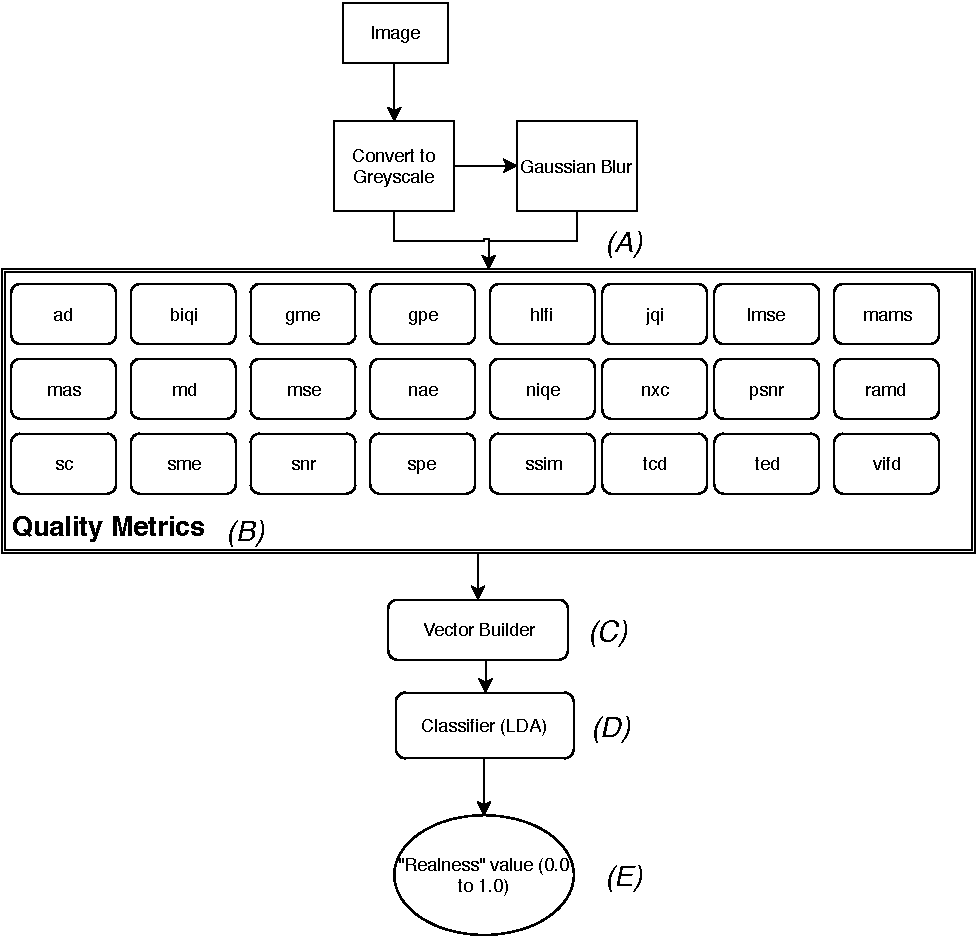
\includegraphics[width=\linewidth]{ImageQualityLivenessTest.pdf}
            \label{ImageQualityLivenessTestDiagram}
            \caption{The architecture of the image quality liveness test. (A) The greyscale copy of the image, and a blurred copy of the image are input into each of the metrics.
            (B) The metrics are individually calculated, and a single value output from them. (C) These values build a 1D vector. (D) They are classified using an LDA classifier. (E) The realness value
            is 1.0 for real, and 0.0 for fake, or in between.}
        \end{figure}

        Originally, the source code accompanying this paper was written in Matlab, using some Matlab-based libraries for certain metrics. Scikit learn provided 
        the necessary classifiers (LDA, SVM), OpenCV provided some simple image manipulation code (e.g. Gaussian Blur), and Numpy allowed for a large amount of
        image-based calculations.

        \paragraph{Numpy/OpenCV powered metrics, utilising image based calculations}
        Several metrics simply required pixel based calculations between an image, and a gaussian blurred version of the same image. These were fairly easy to implement,
        utilising numpy to manage the individual pixel calculations. In some cases (e.g. GradientMagnitudeErrorMetric), other image operations such as a Sobel filter were needed, and in this
        instance OpenCV was used to carry out these operations. Some of these also relied on other linear algebra libraries built into Numpy for the calculations.
        In some cases, further functions were written to work with these libraries.

        Metrics that are included here are: Average, Maximum Difference, Gradient Magnitude Error, Gradient Phase Error Metric, JPEGQualityIndexMetric, MSE (and the laplacian equivalent), Angle-based similarity metrics,
        Absolute Error Metric, Normalised Cross Correlation, Signal to Noise Ratio based metrics, Corner and Edge based metrics, and Visual Information Fidelity metric (which uses gaussian blurs at various scales).

        \paragraph{Fourier/wavelet based metrics}
        In some cases, fourier transforms could be carried out with a combination of opencv and numpy metrics, this was the case with the HighLowFrequencyIndexMetric,
        and SpectralPhaseErrorMetric.

        Some metrics required further wavelet transforms that weren't available within existing imported libraries. Rather than implementing these metrics completely
        from scratch, a library was needed. Existing code had been written \cite{VideoQualityOriginal}, but it had two problems: it wasn't compatible with Python3, but only
        with Python2, and also it wasn't in an easily importable/managable library form for integration into an existing app.

        Therefore, the existing code was forked in order to be updated. The Python2 to Python3 upgrade was completed fairly easily, simply by correcting imports that were incorrect
        for newer versions, and also version specific corrections (such as $== None$ being changed to $is$ $None$ in Python3).
        
        Once this was completed, the code was bundled into a package by creating a $setup.py$ file. This allows for code reuse, and also makes dependencies for the project
        more managable by using a hosted version of the package, rather than a version on the local repository (as the underlying code for the metric will rarely be touched).
        The setup file also requires a Makefile be created to install dependencies using pip. Once this was completed, a GitHub release was created for the package, which allows it to be
        imported into an existing project using pip. \cite{VideoQualityUpdated}. This code implements the VIF, SSIM and NIQE metrics.\todo{Need to adjust how we specify metrics and what they are}

        However, this didn't include all metrics, as the Blind Image Quality Index still wasn't implemented. Once again, there were no Python3 implementations, and only Python2 implementations existed.
        The metric itself calls for running input through a pretrained SVM, using libsvm based libraries on the system. An updated version of pywavelet is used to conduct wavelet transforms, and rather than using sklearn for SVM classification
        running a subprocess is the best solution (reading and writing to a file, and using the data this way). Performance wise this isn't ideal, and the libsvm-based classifier could in the future be
        imported to Sklearn, but it performs adequately for a proof of concept.

        Another final metric that's missing is the RRED metric, as this wasn't implemented. The metric requires the use of steerable pyramids, which have no existing Python implementation, only a Matlab one. In order to implement this metric, it would have required first implementing a steerable pyramid library
        before continuing to implement the remaining metric using this library, for minimal performance benefits of the current system. Therefore, this metric was skipped. \cite{RRED}


    \subsection{Residual Network based 2D liveness test}
        Recently, 2D convolutional neural networks have had great success in image classification tasks. Therefore, it might be possible to train
        a residual neural network (resnet) to classify for facial liveness tasks.

        In order to simplify the process of training, an existing resnet model (ResNet50) was used, with only the final convolutional layer being
        set to trainable. This is because the initial convolutional layers contain the standard features contained within images, while the final one
        learns bundles of features. Internal feed forward activations use relu, while the external output uses the sigmoid activation function

        Initially, I was using the Standard Gradient Descent optimiser, due to the findings of \cite{SGDBetterThanAdamForImageClassification} which stated
        that SGD was better than Adam for generalisation. However, after experimenting further I found that using an Adam optimiser with a learning rate of 0.001
        led to an improved validation accuracy. With SGD the validation accuracy fluctuated, peaking at around 0.75 without increasing further. With Adam, the
        validation accuracy obtained in the results section was yielded, which was quite a large improvement.

        Initially, the entire image was fed directly into the Residual Network, but this yielded fairly poor performance and generalisation. As a result,
        a HoG based face detector was used to find the largest bounding box in an image (of a person's face), and crop the image around this face structure. The HoG detector was
        initially used due to performance benefits, since a neural network based face detector would require slightly more processing power, and therefore time, to both train and
        predict with our model.

        The image is then resized to the expected input size (required for the Keras image data generator), before again being resized to an image of shape (224, 224).
        While this worked, the bounding box width and height ratio did differ a large amount, which could potentially have yielded slightly poorer performance.
        Given a bounding box $B = (top, bottom, left, right)$, we can create a new bounding box $B'$ which retains square dimensions, by first finding the square
        side width $s$. Mathematically, this is defined as:

        $$s = Max(bottom - top, right - left)$$

        Now we create a new bounding box, defined as:

        $$B' = (top, top + s, left, right + s)$$.

        By following this method, the model appeared to perform better overall, as rather than focusing on the overall image quality (which the previous model did),
        it would focus on the facial region.

        During the process of training, it was noted that the HoG detector was missing approximately one eighth of the faces, therefore outputting the entire image, which
        could potentially have an impact on training and the accuracy of the model. Changing this to the CNN based classifier had surprising results: the computational performance increased,
        due to the underlying GPU acceleration, and the accuracy also improved due to the lack of random noise in the training set (through the generators). One thing to note with the CNN based
        face detector was to ensure upsampling was set to zero, otherwise memory issues would result (since the model and face detector model all need to be stored in GPU memory).
        
        All of this massively improved the result, but generalisation was still a concern. Batch Normalization was therefore added to help make the make the model generalise further.
        This yielded a much better result, despite taking slightly longer to train. 

        Throughout the training process, a binary crossentropy loss function was used, since there are only two possible classes, being predicted with a single number output. 

        The final architecture can be seen in Figure \ref{2DCNNArchitecture}. While normalization layers aren't visible, they are located in between each dense layer. The residual network
        is also simplified.

        \begin{figure}
            \centering
            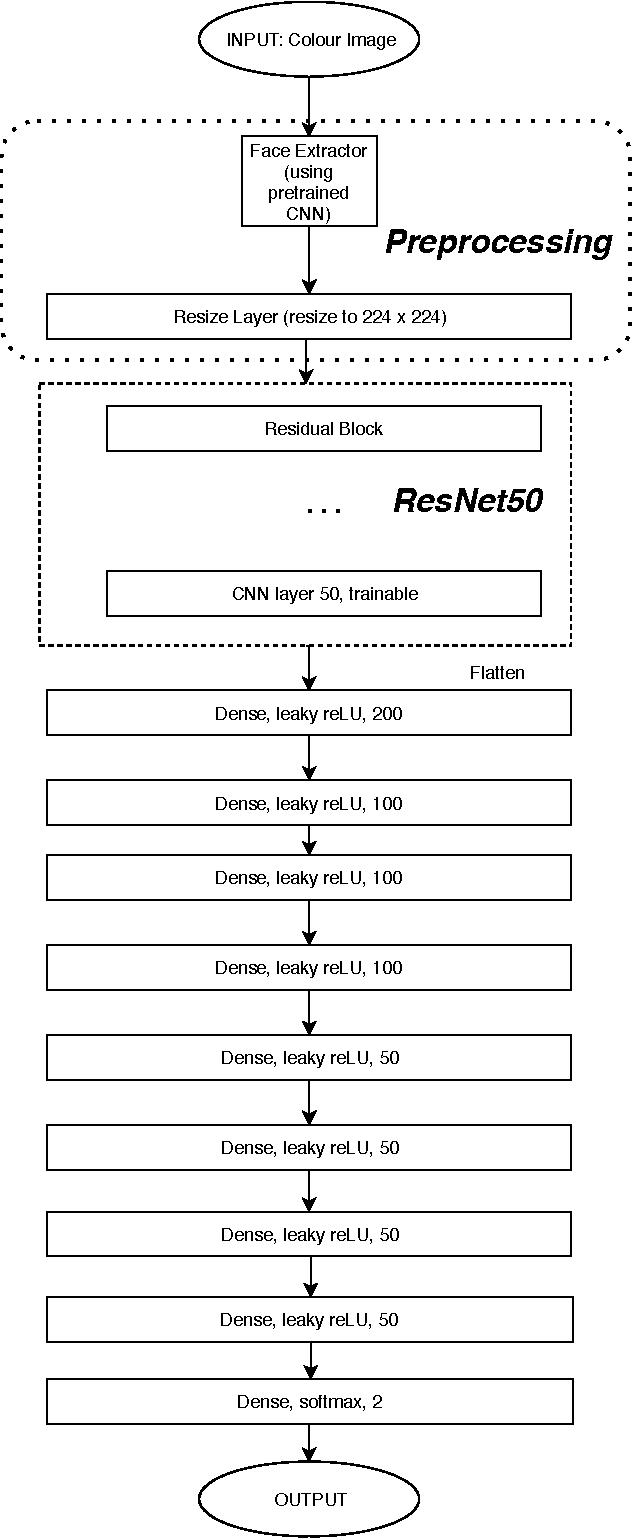
\includegraphics[width=0.6\linewidth]{2DCNNArchitecture.pdf}
            \label{2DCNNArchitecture}
            \caption{The 2D CNN test architecture. We take the face image, resize to a fixed size, and put through ResNet50. The two last CNN layers
            of this ResNet are trainable. The output of this network is flattened and fed through a deep feed forward network, yielding one output (which is the
            liveness score as before).}
        \end{figure}
        \todo{TODO: insert citation for trying pretrained imagenet}

    \subsection{A system for preventing 3D spoofing attacks}
        While the systems before might go partially towards preventing 3D spoofing attacks, though primarily considering the 2D image, we now propose a method
        that is designed for classifying facial liveness based on a 3D point cloud.

        \subsubsection{2D to 3D Conversion}
            In order to classify an image/video, the 2D image needs to be converted to a 3D representation of a user's face. While 3d reconstruction is easier with videos (using structure from motion or other multiview based methods),
            there also exist image-based reconstruction methods such as vrn (\citealt{3DReconstructionMethod}) which are more specific and designed for reconstructing faces based on images. This also has benefits, as structure from motion
            is unable to reconstruct 3D from a single image, or from videos with very little motion.

            The image was converted by first applying a facial detection algorithm on the image, and cropping the image down to provide only the face. This cropped image was then resized to
            be of size $(192, 192)$, still in colour. This cropped and resized image was then fed through the VRN network. After this, the network output was filtered and stacked to provide the voxel input required.

            The code to operate this can be found under the \emph{liveness.vox.reconstruction} namespace within the code.

        \subsubsection{3D point cloud classification}
            Once the 3D reconstruction is obtained, one can then classify this using some model to produce the fake/real metric.
            
            VoxNet takes in a point cloud and converts this to an occupancy grid. This is then fed through two convolutional layers,
            pooled, and then goes through a dense layer before reaching the classifier output (a dense layer with the k outcomes). 

            As a pretrained version of VoxNet wasn't readily available, the whole system was trained together from scratch.

        \subsubsection{Linking everything together}
            While each system is self-contained, linking them together took a little bit more work than expected. The models themselves couldn't be directly joined together,
            as VRN required extra postprocessing steps which couldn't be implemented using tensors within tensorflow. As such, the initial 2D to 3D conversion was required to be run
            as a preprocessing step.

            To assist in the training phase, a generator was written in Python to conduct the postprocessing on the fly for each batch, which didn't require the entire preprocessing step to be done before training, 
            thus reducing the peak memory usage problems. While an ImageDataGenerator was used previously, this isn't compatible with 3D, and therefore a custom module needed to be written.

            Once the preprocessing had been completed, the preprocessed image was fed to the VoxNet. 

            % tODO explain experiments.

            \begin{figure}
                \centering
                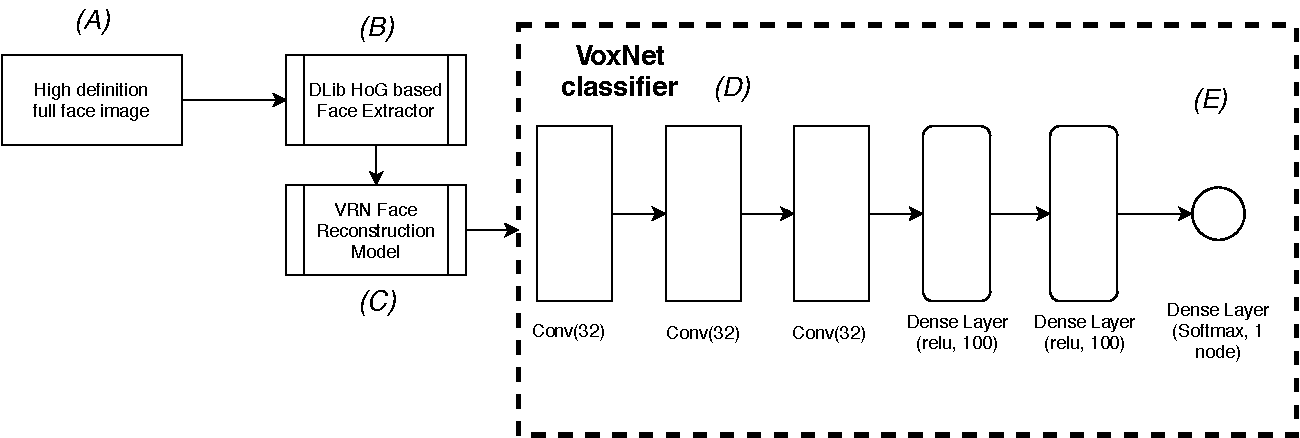
\includegraphics[width=\linewidth]{voxnet.pdf}
                \label{3DClassifierArchitectureDiagram}
                \caption{
                    This is an overview of the 3D classifier. \textbf{(A)} a high resolution image is input into the classifier. \textbf{(B)} The image goes through a HoG based face detector. The bounding box of the face is extracted, and the image is cropped. 
                    The image is then resized to be 192x192 pixels, which is what's required by the VRN process.
                    \textbf{(C)} The pretrained VRN face reconstruction model takes an image input, and outputs a voxel representation. Some postprocessing from the VRN model 
                    is necessary to convert an occupancy grid into a voxel representation (this is done here rather than in the VoxNet model).
                    \textbf{(D)} The VoxNet classifier uses several 3D convolutional layers, along with a couple of Dense layers to classify.
                    \textbf{(E)} The output of the last dense layer is simply a single number defined as the certainty of realness. 1.0 implies the model is certain that the input is real, while 0.0 implies the model is certain that the input is faked.
                }
            \end{figure}

    \subsection{Datasets for training and testing}
            With each of the above classifiers, they were trained using the NUAA dataset (the entire dataset), and the testing was carried out using the Replay-Attack dataset.
            Initially this role was switched, but NUAA has far more samples which makes it more suitable for deep learning classification compared to Replay-Attack.

            Since the Replay-Attack dataset consists entirely of videos, each video was stepped through and an image was produced each second. This was then fed through to the appropriate model.
            
            \todo{Mention more detail here, and cite more information about our implementation e.g. with H5Py for caching, the use of generators for testing/training}

    \subsection{Visualisation and Demonstration}
        In order to visualise the overall outcome of facial liveness, a generic model 
\section{Results}
    % based on the solution, what results did we yield? What did we find out?
    For both liveness tests, cross dataset validation/testing was conducted. Each model was trained using the entire NUAA dataset, and the Replay-Attack test set
    was used to measure the results shown below. In the case of the 2D Convolutional Neural Network (CNN), a validation set was required to ensure the model performed
    well, so in this case the Replay-Attack devel set was used. It must be noted that no overlap occurs between the Replay-Attack devel and test sets, to prevent the risk
    of these results being invalid.

    \subsection{Image Quality Liveness Test}
        Overall, the Image Quality Test performed as expected with reference to the initial paper. Unlike the original paper however, instead of isolating the face
        from the input image, the entire image was used. While isolating the face might perform well, using the entire image might provide further subtle information
        about the image quality.

        \todo{Add False Positive/False Negative accuracy here}
        \todo{Add time to conduct computation here (without multithreading) - for predictions only, not training}

        \todo{show an example image of the system at work with image quality liveness}

    \subsection{2D Convolutional Neural Network Liveness Test}
        \todo{Insert time here to isolate face/preprocess}
        \todo{Insert time here to conduct neural network prediction}
        \todo{Insert system performance (specs of Lexo)}
        \todo{}

        While these results might not appear to be as ideal, this is partly due to the nature of the Replay-Attack dataset as each 20th frame was taken from the dataset.
        Due to this, when there is movement and where the face isn't visible by the camera, the image can't be correctly processed and therefore the entire image is used
        as the input to the network, thus yielding poorer performance than expected. This is only encountered with this metric due to the requirement that the facial extraction is successful. 
        
    \subsection{3D VoxNet Liveness Test}
            As discussed in the method, this metric had several performance challenges. Applying VoxNet caused memory issues, in addition to yielding very poor performance
            (50\% accuracy with a single dense layer output), indicating that the features weren't being learnt correctly. 69\% accuracy was expected, as specified in the
            VoxNet paper \cite{VoxNetModel}. There are a few reasons why this wasn't matched: firstly, the voxnet model we needed required large inputs: (192 x 192 x 192 x 3),
            which is far too high for easy and real-time computation. 

\section{Evaluation}
    % How well our system works, how well did it assess stuff, and how it can be improved.
    % what are the uses of our research? e.g. influence and improve the design of xyz...
    \subsection{Improvements}
    \paragraph{Representing 3D Attacks}
    While our system works fairly well for 2D based attacks, performance for 3D based attacks definitely needs work.
    While our VoxNet based method didn't yield any meaningful results, there is a chance that a 2D image could yield results
    with 3D based attacks (using a residual network on a static image to detect minor mask-based imperfections), or alternatively
    considering a sequence of images using LSTMs to detect changes in movement. This however would require video input, meaning the
    NUAA dataset wouldn't be useful.

    \paragraph{Dealing with source quality attacks that use holes in web browsers}
    Furthermore, while our current system focuses mostly on the liveness tests, one must also consider input-based attacks (using prerecorded digital files
    sent to the server). In the case of the Safari web browser on iOS, existing web browser APIs only allow a general media capture command (which allows the user to
    either record a video/image or upload something from their library), and this can't be overridden. This needs to be addressed in order to provide a truly useful
    liveness service. Video-based tests involving random movement (e.g. head movement) could be added to our consolidation layer to assist in preventing this. Additionally, content ID
    based liveness checks could be used to ensure videos aren't reused, but this would require additional data storage which wouldn't necessarily scale as easily.

    \todo{Mention the GetUserMedia API that is used}
    \todo{Source from https://developer.mozilla.org/en-US/docs/Web/API/MediaDevices/getUserMedia regarding the security aspects }
    \paragraph{Existing BIQI implementation}
    Currently, the BIQI implementation requires the use of a subprocess to call libsvm based commands on the system. Instead of using standard output, files are used which
    cause a reduction in speed.
    \todo{ADD Calculations here for speed with hard drive, SSD, and memory}.
    Speed isn't the only problem here, as scaling would become a problem due to the existing implementation. 

    To fix this problem, a reader would be needed to import a trained libsvm model into sklearn, and the code would then need to be refactored to use the updated sklearn model. 
\section{Conclusions}
    % overall, what did the project show?
    This project showed that creating a facial liveness service for the web is a feasible idea, and performs fairly well for 2D attacks. The consolidation layer provides
    an ideal point of extension, allowing for multiple tests to work together and allow confirmation to prevent false positives (which would lead to security problems).

\bibliographystyle{plain}
\bibliography{report}

\end{document}